\documentclass[float=false, crop=false]{standalone}
\usepackage[subpreambles=true]{standalone}
\begin{document}

\subsection{Entwicklung}
\label{sec:entwicklung}

Das Resource Description Framework (RDF) wurde ursprünglich 1999 vom World Wide Web Consortium (W3C) als Empfehlung verabschiedet \autocite{Lassila:99:RMS}. 2004 wurde diese Version aktualisiert und in mehrere Dokumente aufgeteilt \autocite{Beckett:04:RSS}. Die aktuelle, erweiterte Version (RDF 1.1) wurde 2014 veröffentlicht \autocite{Schreiber:14:RP}. RDF 1.1, im Weiteren nur als RDF bezeichnet sofern nicht anders festgelegt, hat das Ziel die Unterstützung neuer Anwendungsfelder für RDF zu stärken. \autoref{tab:rdf} zeigt die Erweiterung von RDF 1.0 auf RDF 1.1 (vgl. \cite[Abs.~2]{Klyne:04:RDF}; \cite[Abs.~2]{Schreiber:14:RP}; \cite{Wood:14:WNR}). Davon kann man ableiten, dass RDF sich in die Richtung entwickelt, immer mehr domänenspezifische Anwendung zu unterstützen. Das bedeutet, dass kleinere Unternehmen mit vereinfachte JSON basierte REST-APIs Datenintegration\footnotemark{} auf die syntaktischen und semantischen Ebene anhand RDF wirksam einsetzen können.
\footnotetext{vgl. die semiotische Ebenen der Integration in \citeauthor{Schissler2004}}

\begin{table}[h]
	\centering
	\begin{tabular}{|p{9em}|c|c|}
		\hline \rule[-2ex]{0pt}{5.5ex} Anwendungsfall & RDF 1.0 & RDF 1.1 \\ 
		\hline \rule[-2ex]{0pt}{5.5ex} Web-Metadaten & RDF/XML & HTML5+RDFa 1.1, JSON-LD\\ 
		\hline \rule[-2ex]{0pt}{5.5ex} Datenaustausch zw. Datenbanken\footnotemark{}& RDF/XML & JSON-LD, TriG, N-Quads  \\
		\hline \rule[-2ex]{0pt}{5.5ex} API-Feeds Verbinden \footnotemark[\value{footnote}] & RDF/XML& JSON-LD, RDF/XML\\ 
		\hline
	\end{tabular}
	\caption{Die Entwicklung von RDF}
	\label{tab:rdf}
\end{table}
\footnotetext{vgl. \cite[Abs.~2]{Klyne:04:RDF}; \cite[Abs.~2]{Schreiber:14:RP}; \cite{Wood:14:WNR}}

\subsection{Beschreibung} 

Laut \citeauthor{Schreiber:14:RP} in \citetitle{Schreiber:14:RP}: 

\hyphenblockquote{german}{RDF is intended for situations in which information on the Web needs to be processed by applications, rather than being only displayed to people. RDF provides a common framework for expressing this information so it can be exchanged between applications without loss of meaning.} 

Wie der Name vermuten lässt, bietet das Resource Description Framework ein Gerüst (Modell, Sprachen und Syntaxen) für die Beschreibung von Attributen, Funktionen und Beziehungen der Ressourcen. Ressourcen können alles sein, was einen einzigartigen Identifier (URI oder IRI) hat \autocite[vgl.][Folie~6]{Dekeyzer2013}. RDF legt eine abstrakte Syntax fest um Zusammenhänge zwischen Ressourcen als eine Menge gerichteter Graphen darzustellen. Ein gerichteter Graph (genannt \hyphenquote{german}{Triple} in RDF) hat einen Knoten (Subjekt), der über eine gerichtete Kante (Prädikat) mit einem anderen Knoten (Objekt) in Verbindung steht. \autoref{fig:rdf-intro} veranschaulicht die abstrakte Syntax von RDF. Das Beispiel\footnotemark{} drückt die Beziehung zwischen einem Kartograph und eine gezeichnete Karte aus.

\footnotetext{Das Datenmodell basiert auf einer Web-Applikation (\href{http://kartenlabor.uni-erfurt.de}{Globmaplab}), die für die Arbeit mit den historischen Beständen der Sammlung Perthes konzipiert wurde. Offenlegung: der Autor dieser Arbeit war Lead-Entwickler dieses Projekts.}

\begin{figure}[h]
	\centering
	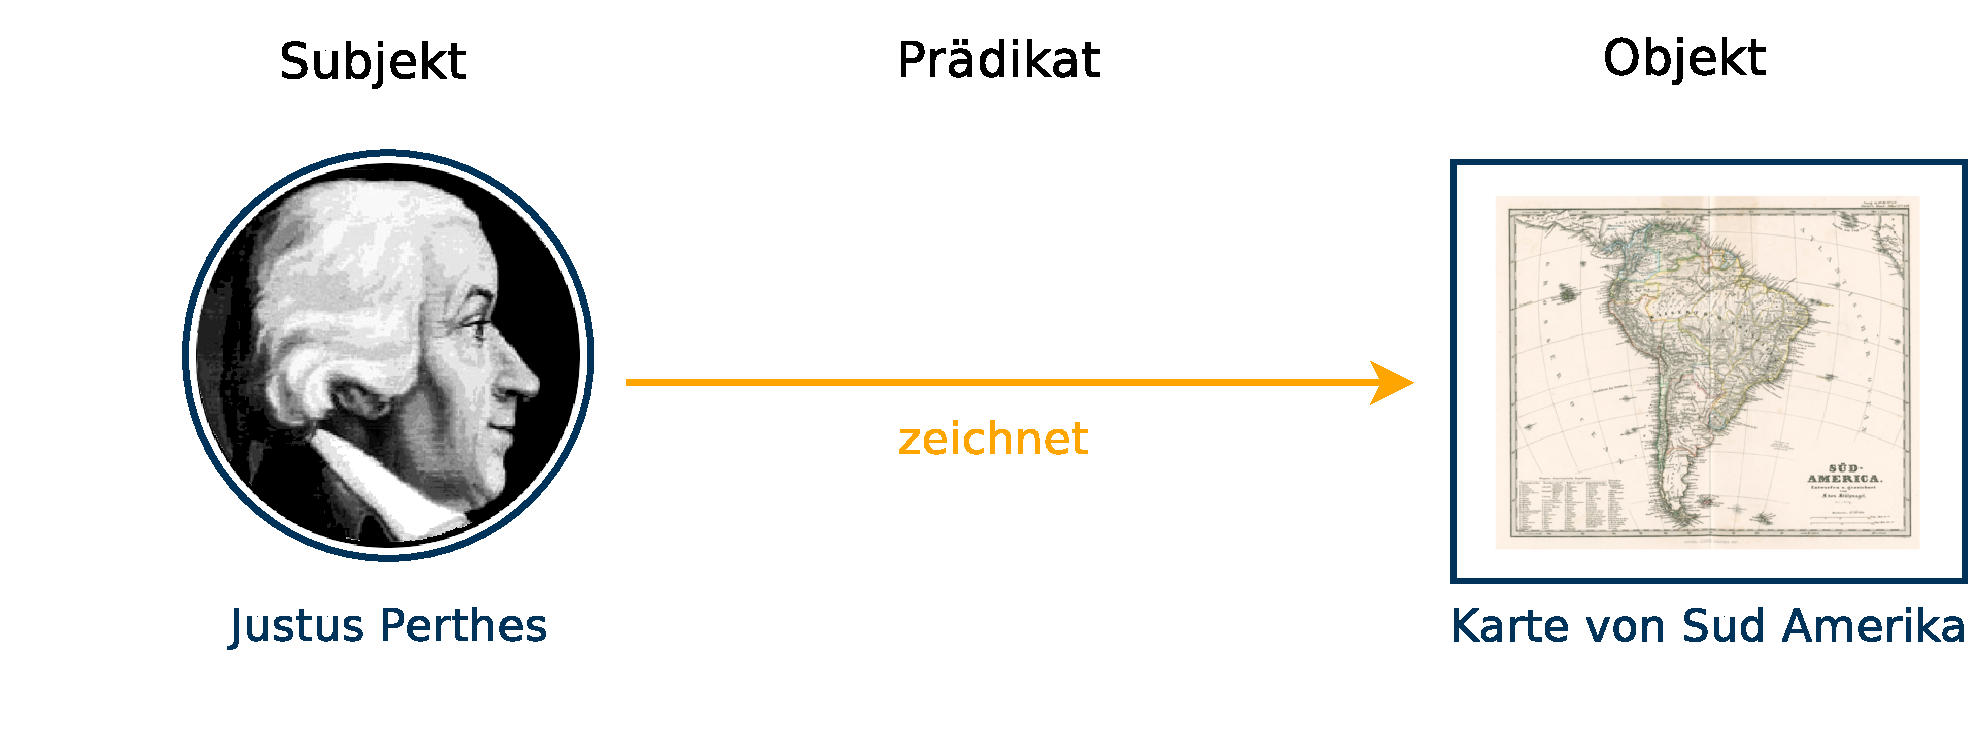
\includegraphics[width=1\linewidth]{images/spo}
	\caption[Kernkonzepte des RDFs]{Kernkonzepte des RDFs}
	\label{fig:spo}
\end{figure}

Jede Komponente eines RDF-Tripels kann eine von drei Ausprägungen haben \autocite[vgl.][Abs.~3.1]{Wood:14:RCA}.

\begin{itemize}
	\item Ein Subjekt ist ein \textit{IRI} oder ein \textit{Blank Node}.
	\item Ein Prädikat ist ein \textit{IRI}.
	\item Ein Objekt ist entweder ein \textit{IRI}, ein \textit{Literale} oder ein \textit{Blank Node}.
\end{itemize}

Ein \textit{IRI} (International Resource Identifier, festgelegt in RFC 3987) ist eine Generalisierung eines URIs (Uniform Resource Indicator, RFC 3986), die Zeichen aus der nicht-ASCII Bereich der Universal Character Set\footnote{wie in Norm ISO/IEC 10646 und in \hyphenquote{german}{\href{http://www.unicode.org/versions/latest}{The Unicode Standard}} vorgegeben ist} erlauben (vgl. \cite[][Abs~3.2]{Schreiber:14:RP}; \cite[]{rfc3987}). IRIs können die Eigenschaften haben, durch die Internet und World Wide Web (TCP/IP + DNS + HTTP) global eindeutig und \hyphenquote{german}{dereferenzierbar} zu sein \autocite[vgl.][Abs.~2]{Jacobs:04:AWW}. 

Ein \textit{Literal} ist eine konkrete Ausprägung eines Datentypen (wie z. B. eine Zeichenkette, Zahl oder Datum) und kein IRI. Ein String-Literal kann wahlweise mit einem \hyphenquote{german}{language tag} assoziiert sein, um die beinhaltete Sprache zu kennzeichnen. RDF Literals können alle Datentypen, die in der XML Schema Definition Language\footnote{\url{http://www.w3.org/TR/xmlschema11-2/}} definiert sind, verwenden \autocite[vgl.][Abs. 5]{Wood:14:RCA}. 

\textit{Blank Nodes} sind von IRIs und Literals disjunkt. Diese Abgrenzung macht es möglich Ressourcen, die keine URI haben, in RDF abzubilden. 
\end{document}
